\newpage
\section{Создание Примитивного Проекта с Нуля}

\subsection{Шаг 1. Project Browser}
Первым делом для создания проекта необходимо открыть Unreal Project Browser.

Unreal Project Browser представляет собой конфигуратор для создания новых проектов. 
В нем вы можете увидеть различные шаблоны (например, шутер от первого лица, игра с видом сверху и другие).

Мы выберем пустой (Blank) шаблон с такими конфигурациями:
\begin{figure}[h]
    \centering
    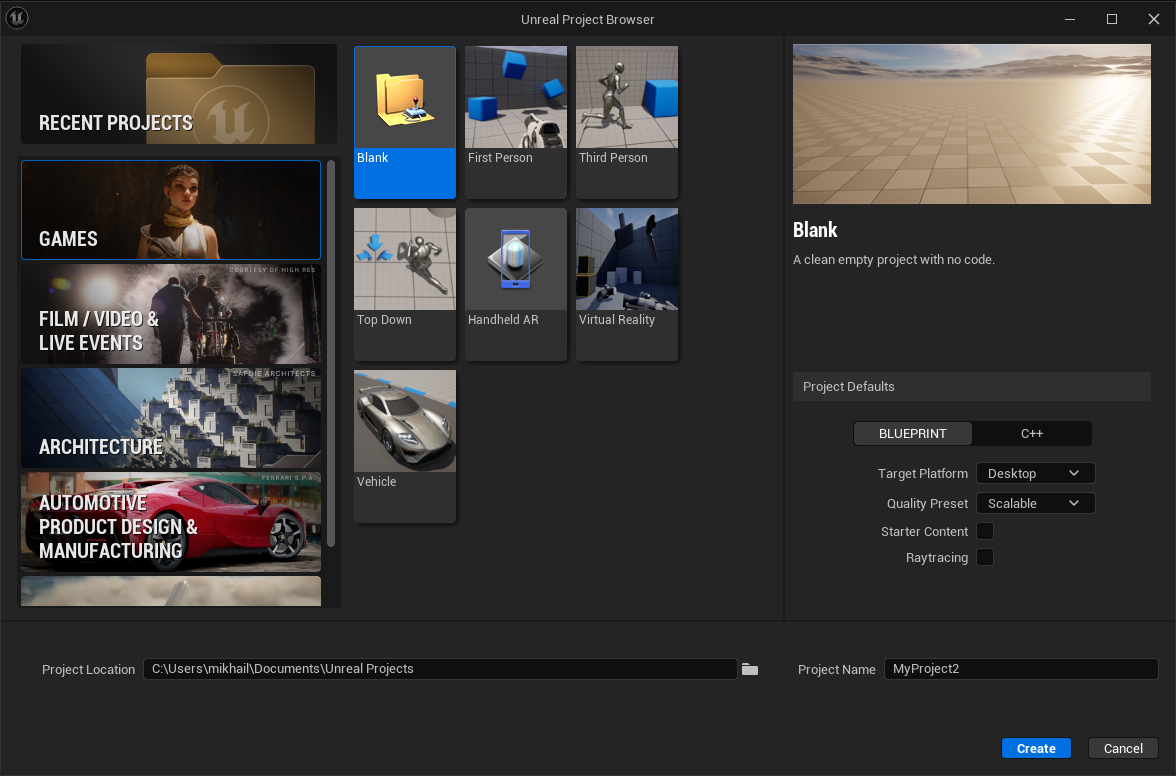
\includegraphics[width=\textwidth]{Lections/ProjectBrowser.png}
    \caption{Интерфейс Unreal Project Browser с выбранным пустым шаблоном}
\end{figure}

\subsection{Шаг 2. Настройка интерфейса и создание уровня}
Для начала установим классический интерфейс редактора через верхнее меню \textbf{Window → Layout → UE4 Classic Layout}.

\begin{figure}[h]
    \centering
    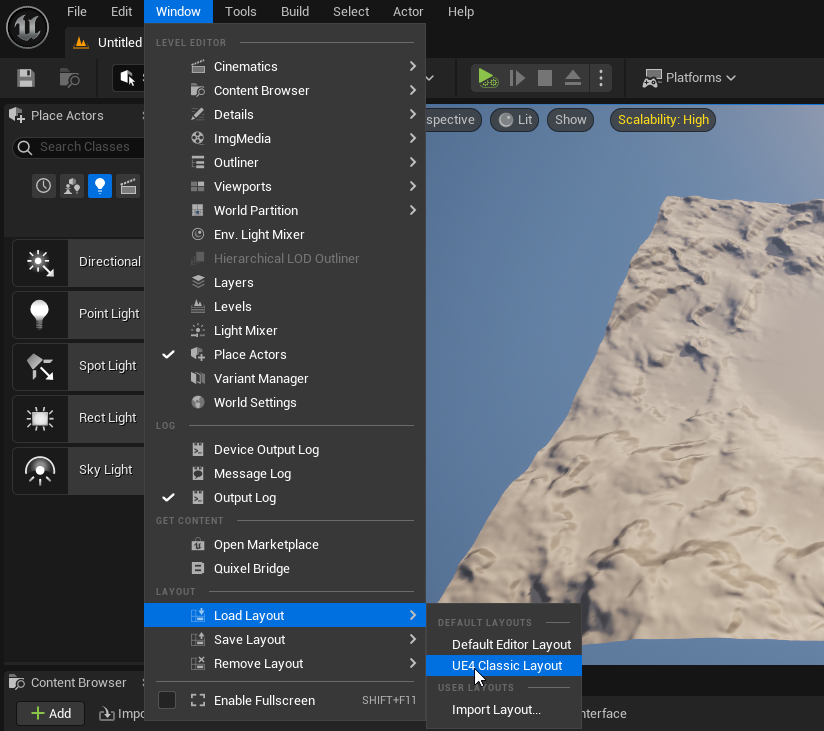
\includegraphics[width=\textwidth]{Lections/Layout.png}
    \caption{Установка классического интерфейса редактора}
\end{figure}

На старте нам дается уровень с большой картой. Давайте создадим новый уровень с упрощенной картой.

В верхнем меню переходим в \textbf{File → New Level → Basic} и нажимаем \textbf{Create}. Теперь нужно сохранить этот уровень в папку проекта с помощью сочетания клавиш \textbf{Ctrl+S}. Для удобства лучше выделить отдельную папку \textbf{Levels} и сохранить новый уровень туда с префиксом \textbf{L\_}.

\begin{figure}[h]
    \centering
    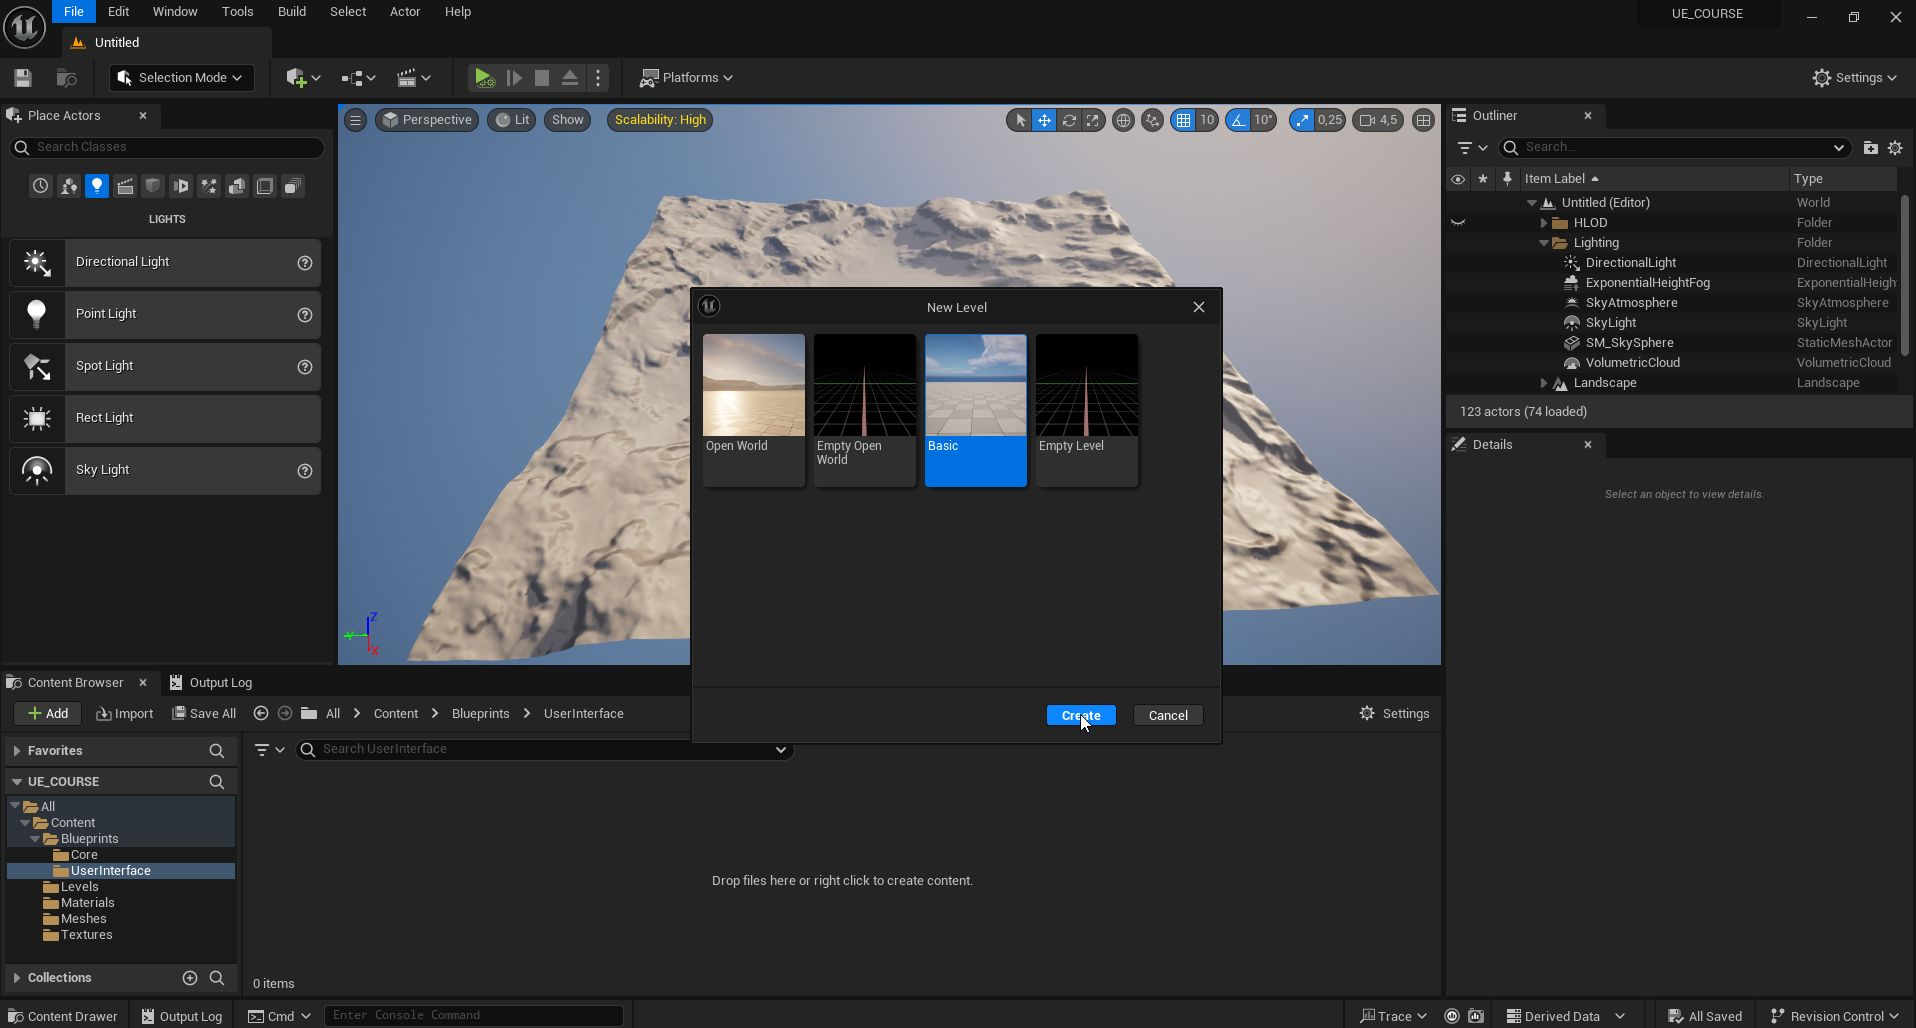
\includegraphics[width=\textwidth]{Lections/LevelChange.jpg}
    \caption{Создание и сохранение нового уровня}
\end{figure}

\newpage

\subsection{Шаг 3. Работа с базовыми объектами}

В классическом отображении интерфейса слева можно увидеть панель \textbf{Place Actors}.

\textbf{Actor} — это любой объект, который может быть размещен на уровне (\textbf{Level}).

\textbf{Actor} состоит из компонентов и может управлять их поведением.

\textbf{Components} (компоненты) — это объекты с определенной функциональностью, которые можно добавить к \textbf{Actor}, чтобы расширить его возможности.

Unreal Engine поддерживает вложенно-агрегированную\footnote{Агрегация — это способ организации объектов, при котором вложенные объекты и основной объект могут существовать независимо друг от друга.} структуру, позволяя подключать компоненты к actor`ам, изменяя функционал и поведение actor`ов.

Примером такой структуры является отношение уровня к акторам, размещенным в нем. Уровень может существовать независимо от actor`ов, размещенных на нем.

Для примера разместим на уровне куб (Cube) из меню \textbf{Place Actors}. Теперь, используя горячие клавиши (\textbf{W, E, R}) или кнопки в окне \textbf{Viewport}, можно переключаться между режимами изменения трансформации (\textbf{Transform}) объекта.

\begin{figure}[h]
    \centering
    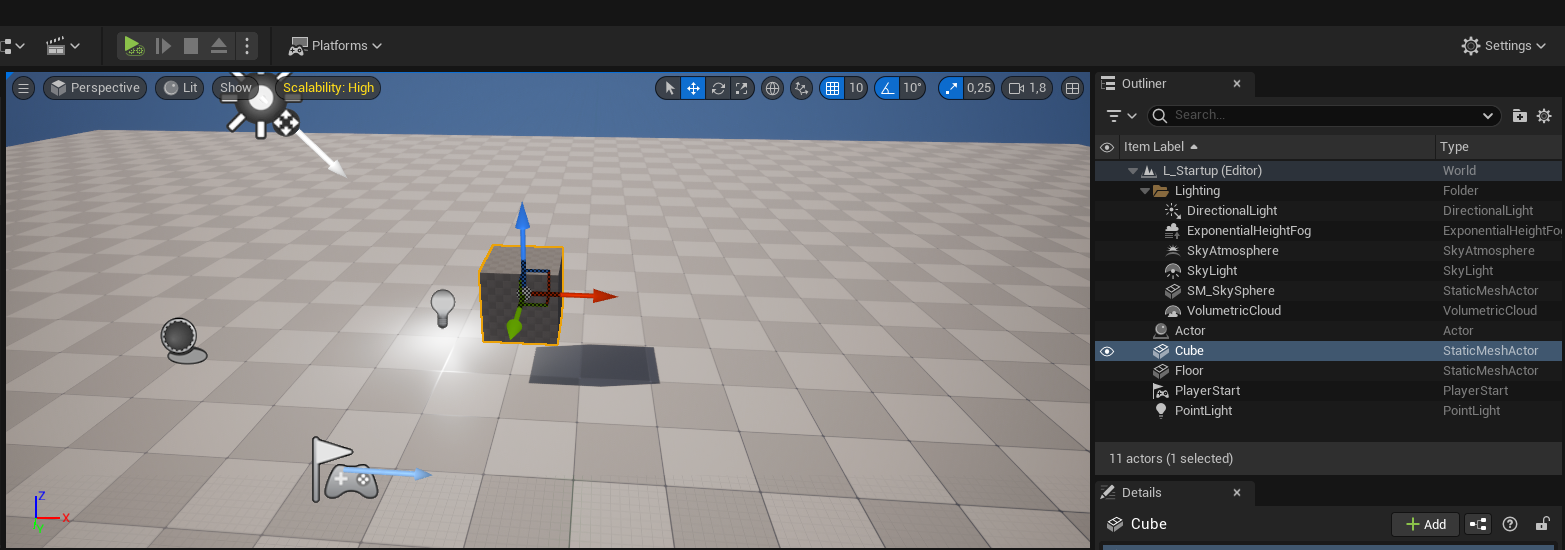
\includegraphics[width=\textwidth]{Lections/LevelAgrigation.png}
    \caption{Пример использования агрегированной структуры с объектами на уровне}
\end{figure}


\textbf{Transform} — это структура, содержащая три вектора (\textbf{Location} — расположение, \textbf{Rotation} — поворот, \textbf{Scale} — масштаб), которые определяют положение и трансформацию объекта в пространстве.

Для изменения других свойств актера можно воспользоваться меню \textbf{Details}.

\textbf{Details} — здесь собраны параметры актера и его компонентов, размещенного на сцене.

Поскольку у компонента \textbf{StaticMeshComponent} есть возможность включения физики, включим её и поднимем куб над полом. Теперь запустим проект в режиме \textbf{Simulate}.

\begin{figure}[h]
    \centering
    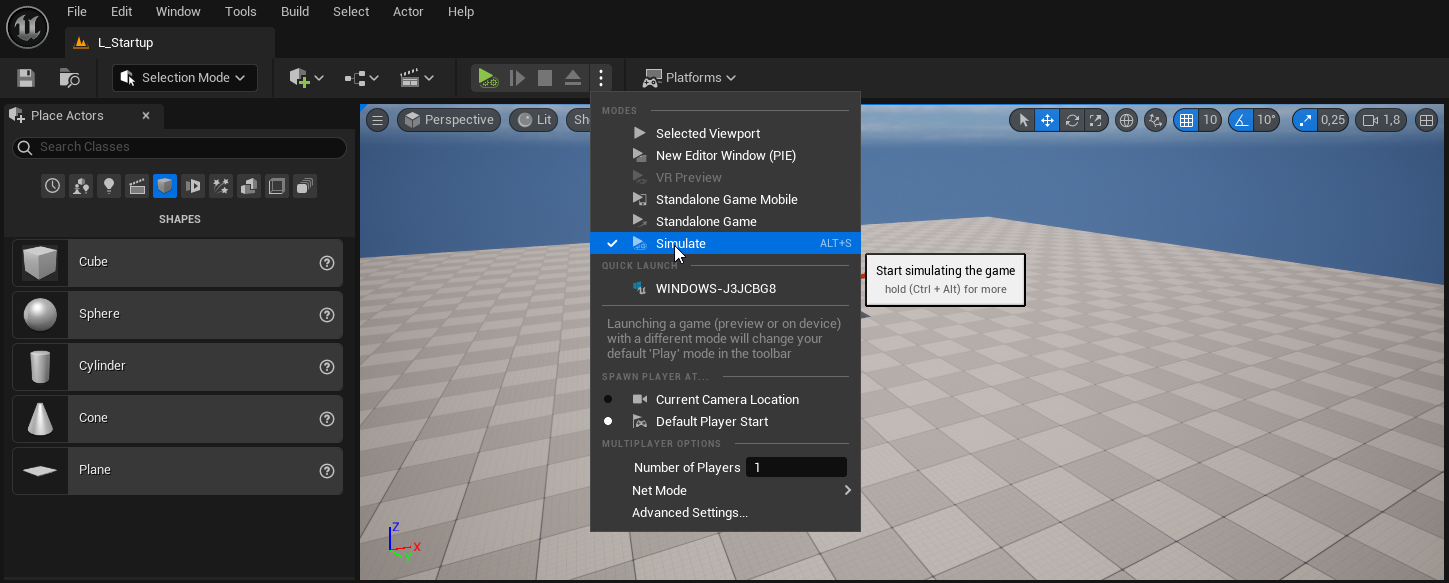
\includegraphics[width=\textwidth]{Lections/StartInSimilate.png}
    \caption{Запуск проекта в режиме \textbf{Simulate}}
\end{figure}

\subsection{Шаг 4. Режимы запуска проекта}

Для тестирования и отладки проекта существует несколько вариантов запуска игры:

-\hspace{1em}\textbf{Selected Viewport} — классический запуск игры в окне Viewport.

-\hspace{1em}\textbf{New Editor Window} — запуск игры в отдельном окне редактора. 

-\hspace{1em}\textbf{VR Preview} — запуск игры в режиме виртуальной реальности (если подключена VR-гарнитура).

-\hspace{1em}\textbf{Standalone Game или Mobile} — запуск в отдельном процессе, имитирующем реальное устройство.

-\hspace{1em}\textbf{Simulate} — запуск в режиме наблюдателя, когда вы видите физическое и логическое поведение объектов.

\subsection{Шаг 5. Базовая логика и Level Blueprint}

Для реализации базовой логики и взаимодействия объектов на уровне используется \textbf{Level Blueprint}. Это визуальный скриптовый инструмент, позволяющий создавать логику без написания кода, связывая различные объекты и их события.

Прежде чем открыть Level Blueprint, стоит напомнить о том, что было сказано ранее. Поскольку структура игрового движка основана на логике вложенности и взаимодополнения, эта парадигма сохраняется и для логики. Каждый элемент в движке имеет свой код и может влиять на другие элементы игрового и неигрового окружения.

Когда мы говорили об акторах (\textbf{Actors}) и их компонентах, мы рассматривали их как отдельные логические единицы, каждая из которых содержит свою логику и может дополнять другие. Но как тогда воспринимать уровень (\textbf{Level}) — как актор или как компонент?

На данном этапе, не углубляясь в ООП\footnote{ООП (Объектно-ориентированное программирование) — это парадигма программирования, в основе которой лежит взаимодействие объектов (сущностей), наделенных набором свойств и методов.}, можно сказать, что уровень является вершиной иерархии игровых объектов. Level содержит акторов, а акторы, в свою очередь, содержат компоненты. 

Таким образом, как высший элемент объектной иерархии, Level получает возможность управлять всеми actor`ами, размещенными в нем.


\begin{figure}[h]
    \centering
    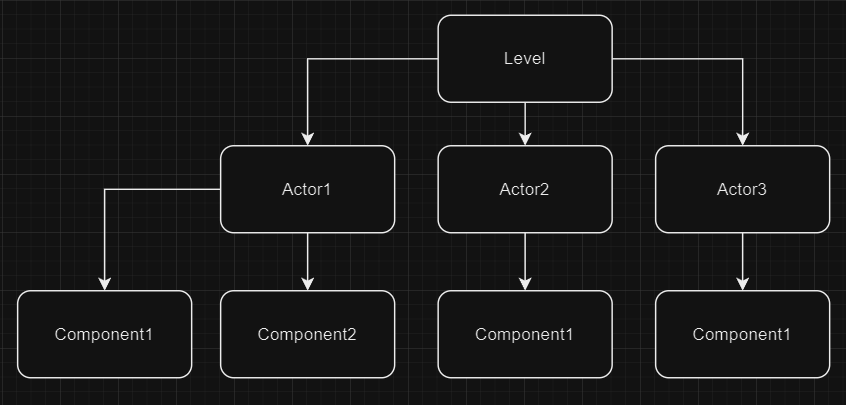
\includegraphics[width=0.75\textwidth]{Lections/BasicStructure.png}
    \caption{Структура вложенности уровня}
\end{figure}

После всего вышесказанноро можем перейти к \textbf{Level Blueprint}.

\begin{figure}[h]
    \centering
    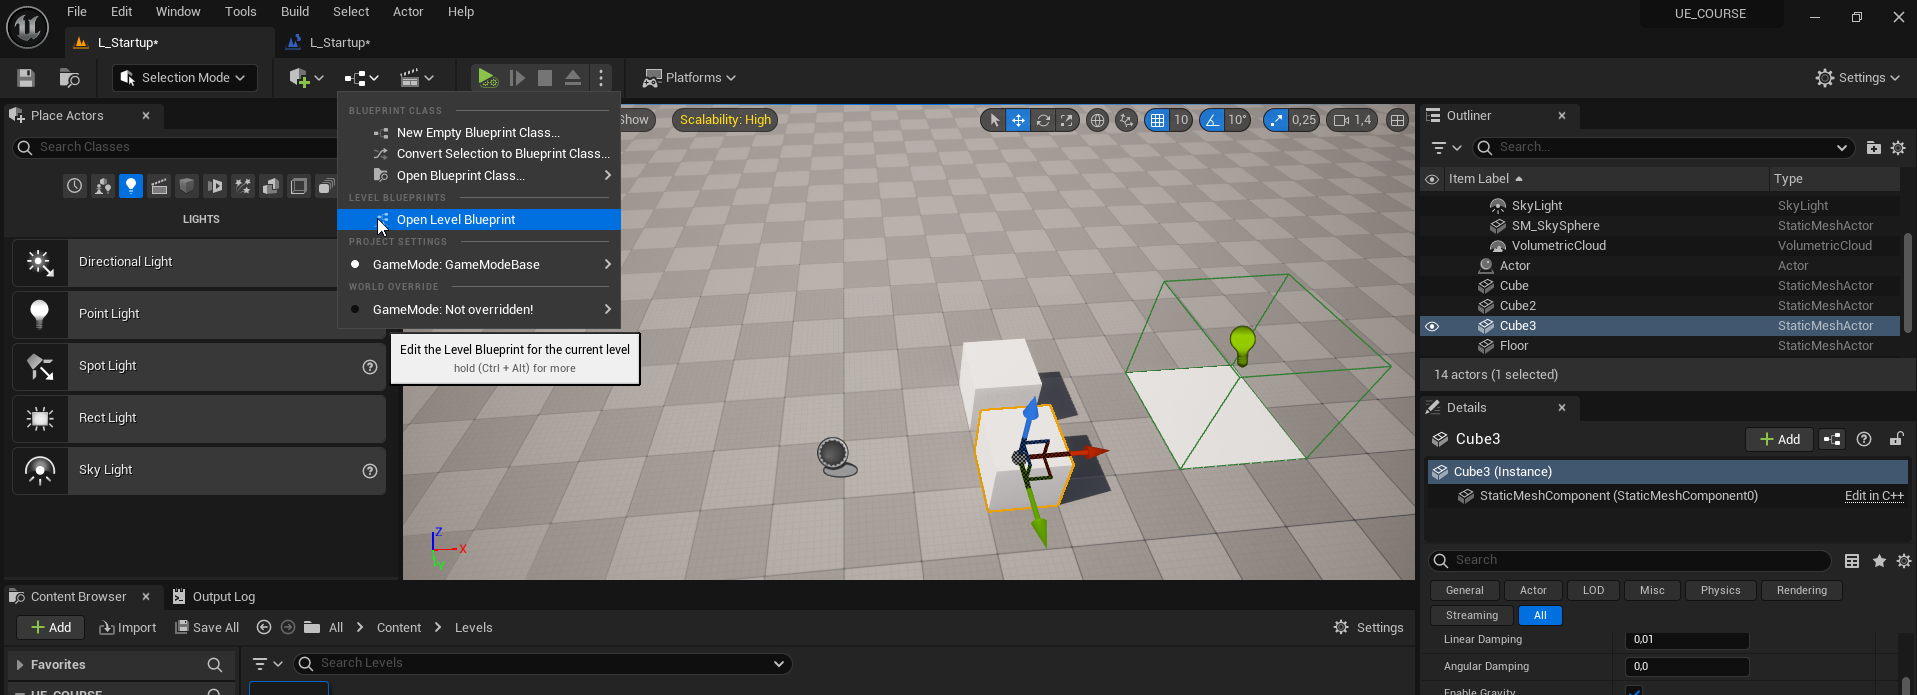
\includegraphics[width=0.75\textwidth]{Lections/LevelBlueprint.png}
    \caption{Level Blueprint}
\end{figure}

\newpage
\subsubsection{Редактор Blueprints}

\textbf{Blueprint (Чертеж)} — это шаблон, содержащий скриптовую логику, описывающую поведение объектов.

Редактор Blueprints представляет собой редактор кода с визуальным программированием. В нем можно создавать функции, переменные и события (\textbf{Events}). Его функционал позволяет описывать логику объекта, компилировать код и отлаживать программу.

\begin{figure}[h]
    \centering
    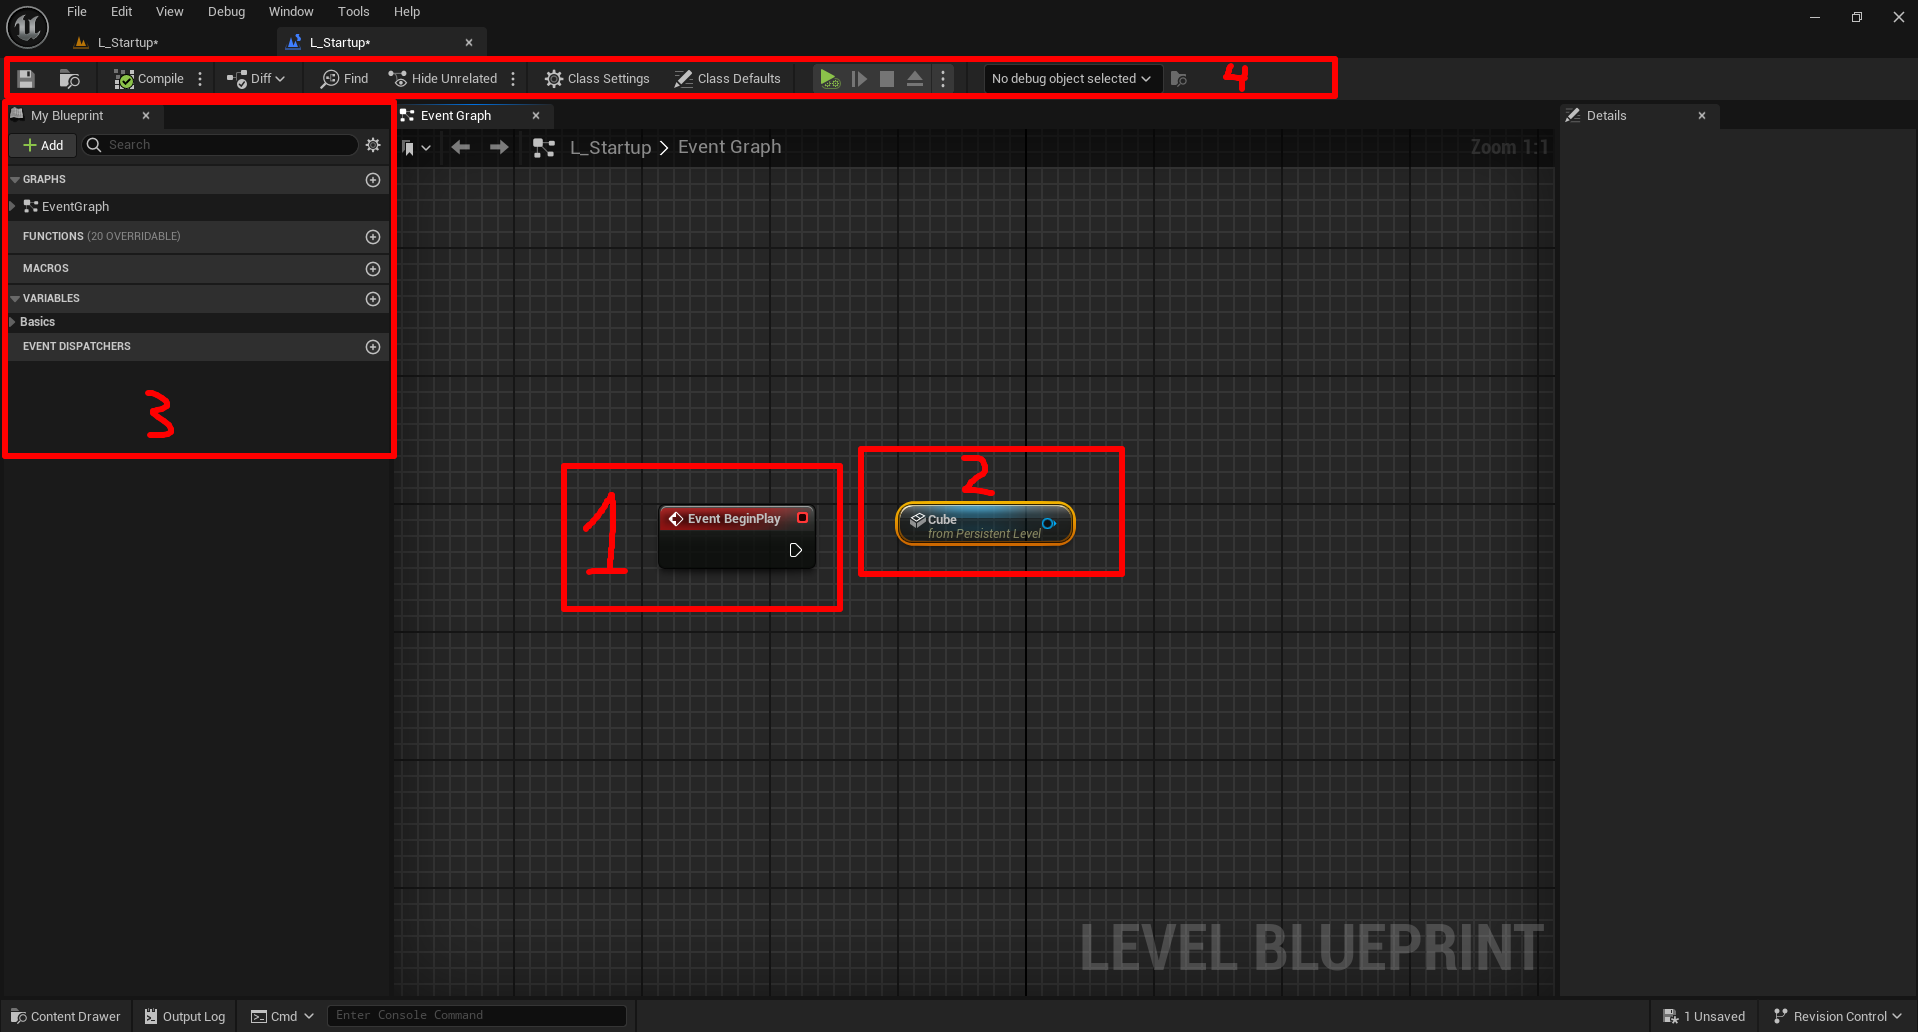
\includegraphics[width=0.9\textwidth]{Lections/BlueprintOverview.png}
    \caption{(1. BeginPlay событие начала игры; 2. Ссылка на куб; 3. Панель MyBlueprint - здесь отображаются основные элементы кода; 4. Панель управления - здесь можно компилировать, отлаживать, и запускать код.)}
\end{figure}

Панель \textbf{MyBlueprint} отражает основные элементы кода, переменные и функции. Также в нем находятся \textbf{Графы (Graphs)}, которые являются окружением для написания кода.

Сверху находится панель инструментов, содержащая основные действующие кнопки: компиляция, сохранение и отладка (\textbf{debug}).

\textbf{Event (Событие)} — это элемент кода, который вызывается actor`ами или внешними системными объектами движка.

\subsubsection*{Сравнение событий Unreal Engine с работой предприятия:}

1.\hspace{1em}Старт предприятия $\rightarrow$ запуск движка (вызов всех конструкторов).

2.\hspace{1em}Все работники на своих местах и готовы приступить $\rightarrow$ завершение инициализации.

3.\hspace{1em}Звонок о начале работы предприятия $\rightarrow$ запуск игры (вызов \textbf{Begin Play}).

4.\hspace{1em}Пока предприятие работает, подгонять работников как можно чаще $\rightarrow$ работа события \textbf{Tick}.

5.\hspace{1em}Завершение работы предприятия $\rightarrow$ вызов события \textbf{EndPlay}.

В редакторе \textbf{Level Blueprint} мы можем обращаться к любым объектам на уровне, менять их свойства и взаимодействовать с ними.

Давайте обратимся к ранее созданному кубу на уровне, отключим физику и выделим его. С выделенным кубом перейдем в редактор \textbf{Level Blueprints}. Правой кнопкой мыши нажмем по пустому полю. В выпадающем меню выберем \textbf{Create a Reference to Cube}.

\begin{figure}[h]
    \centering
    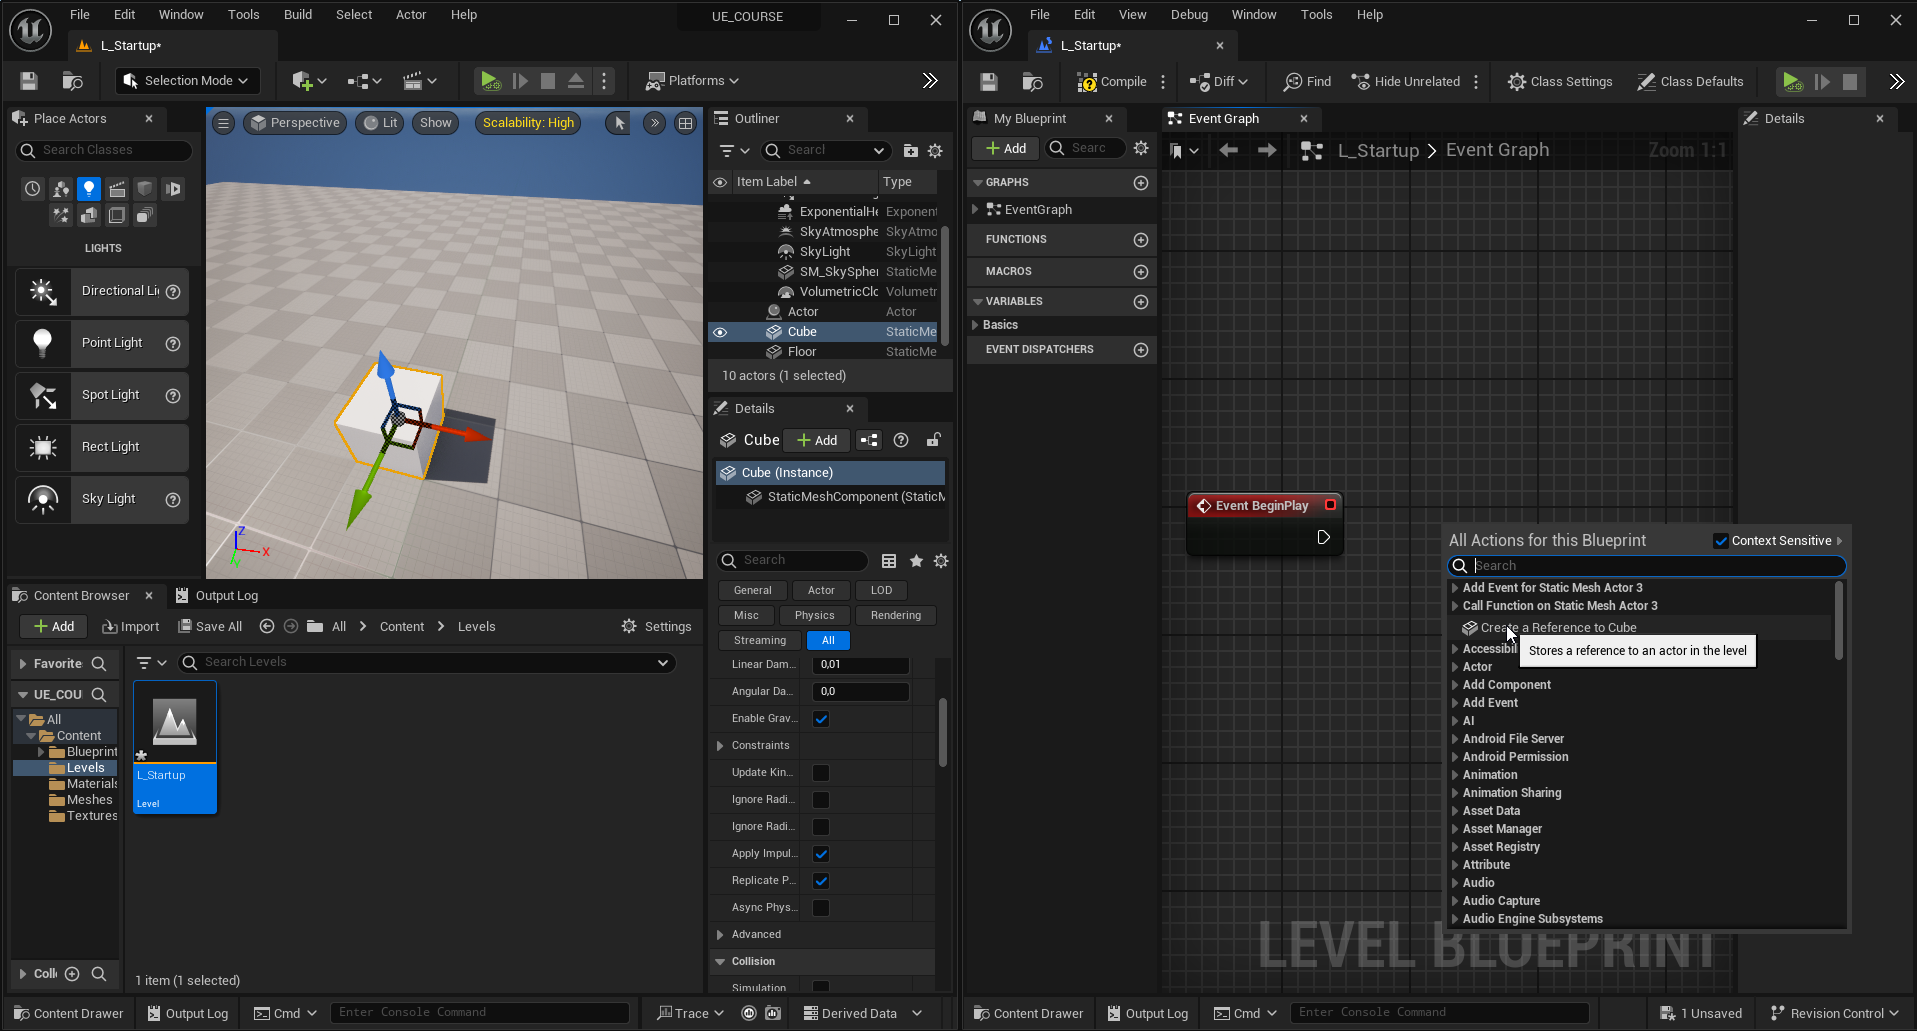
\includegraphics[width=0.9\textwidth]{Lections/CreateReferenceToCube.png}
    \caption{Создание ссылки на куб}
\end{figure}

\textbf{Reference (Ссылка)} — это переменная-ссылка, содержащая доступ к объекту, находящемуся по указанному адресу.

С помощью ссылок на объекты мы можем изменять сам объект и его свойства.

К примеру, уничтожим этот объект с помощью метода \textbf{Destroy} с самого начала игры. Для того чтобы обращаться к методам объекта, нужно потянуть за ссылку и отпустить в пустом поле, чтобы появилось контекстное меню. Далее введем в поиске \textbf{Destroy Actor} и нажмем \textbf{Enter}.

Теперь остается только вызвать этот метод в нужный момент, а именно при вызове события \textbf{EventBeginPlay}. Протянем сигнальный узел от пина \textbf{EventBeginPlay} к пину \textbf{DestroyActor}. Скомпилируем скрипт с помощью кнопки \textbf{Compile}. После запуска в режиме \textbf{Simulate} куб уничтожится.
а
\begin{figure}[h]
    \centering
    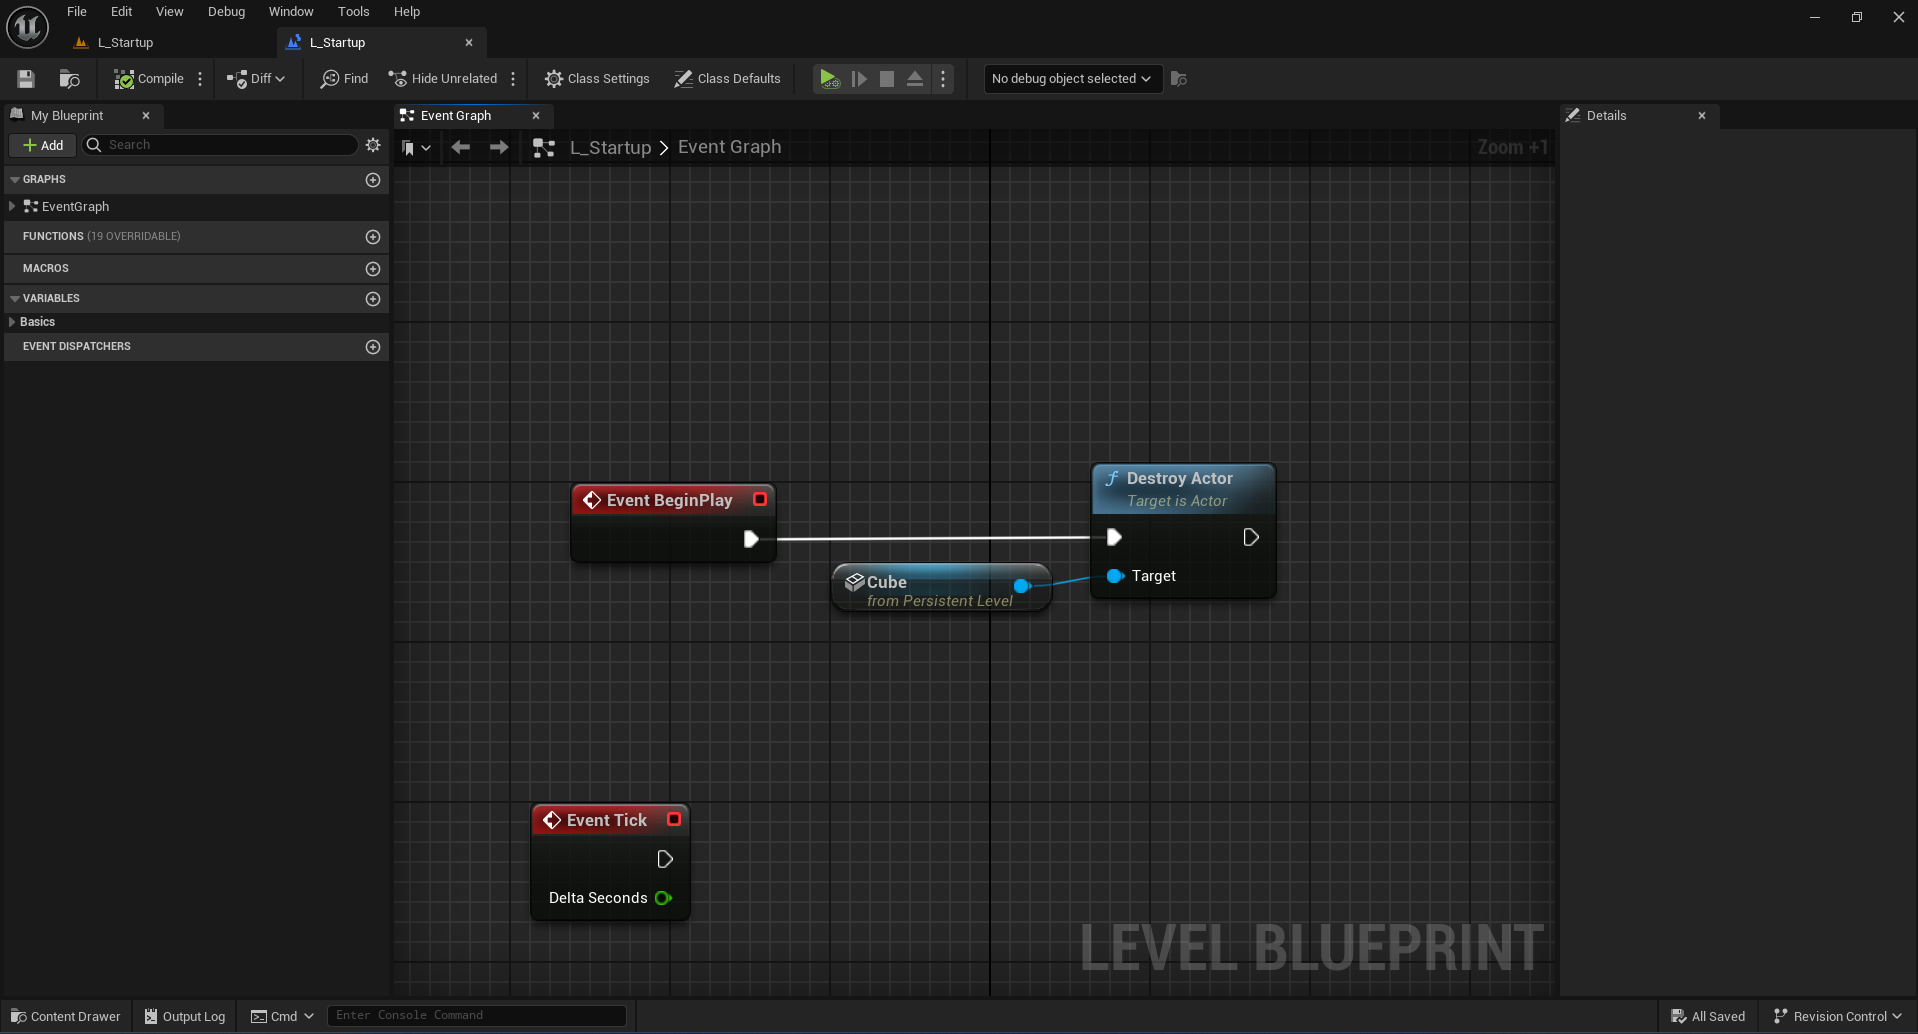
\includegraphics[width=0.9\textwidth]{Lections/DestroyCubeBeginPlay.png}
    \caption{Скрипт уничтожения куба}
\end{figure}

